\documentclass[a4paper,14pt]{extarticle}

\usepackage[utf8x]{inputenc}
\usepackage[T1,T2A]{fontenc}
\usepackage[russian]{babel}
\usepackage{hyperref}
\usepackage{indentfirst}
\usepackage{here}
\usepackage{array}
\usepackage{graphicx}
\usepackage{caption}
\usepackage{subcaption}
\usepackage{chngcntr}
\usepackage{amsmath}
\usepackage{amssymb}
\usepackage{pgfplots}
\usepackage{pgfplotstable}
\usepackage[left=2cm,right=2cm,top=2cm,bottom=2cm,bindingoffset=0cm]{geometry}
\usepackage{multicol}

\renewcommand{\le}{\ensuremath{\leqslant}}
\renewcommand{\leq}{\ensuremath{\leqslant}}
\renewcommand{\ge}{\ensuremath{\geqslant}}
\renewcommand{\geq}{\ensuremath{\geqslant}}
\renewcommand{\epsilon}{\ensuremath{\varepsilon}}
\renewcommand{\phi}{\ensuremath{\varphi}}

\counterwithin{figure}{section}
\counterwithin{equation}{section}
\counterwithin{table}{section}
\newcommand{\sign}[1][5cm]{\makebox[#1]{\hrulefill}} % Поля подписи и даты
\graphicspath{{pics/}} % Путь до папки с картинками
\captionsetup{justification=centering,margin=1cm}
\def\arraystretch{1.3}

\begin{document}

\begin{titlepage}
\begin{center}
	\textbf{Санкт-Петербургский Политехнический Университет \\Петра Великого}\\[0.3cm]
	\small Институт компьютерных наук и технологий \\[0.3cm]
	\small Кафедра компьютерных систем и программных технологий\\[4cm]
	
	\textbf{ОТЧЕТ}\\ \textbf{о лабораторной работе}\\[0.5cm]
	\textbf{<<Исследование частотных характеристик пассивных RC-цепей>>}\\[0.1cm]
	\textbf{Электротехника и Электроника}\\[10.5cm]
\end{center}

\begin{flushright}
	\begin{minipage}{0.60\textwidth}
		\begin{flushleft}
			\small \textbf{Работу выполнили студенты}\\[3mm]
			\small группа 23501/4 \hspace*{17mm} Дьячков В.В.\\[3mm]
			\small группа 23501/4 \hspace*{17mm} Ламтев А.Ю.\\[5mm]
			
			\small \textbf{Преподаватель}\\[5mm]
		 	\small \sign[3.5cm] \hspace*{8mm} к.т.н., доц. Кочетков Ю.Д.\\[0.5cm]
		\end{flushleft}
	\end{minipage}
\end{flushright}

\vfill

\begin{center}
	\small Санкт-Петербург\\
	\small \the\year
\end{center}
\end{titlepage}

\section{Цель работы}

Овладеть методикой расчета и экспериментально исследовать основные параметры однокаскадных транзисторных усилителей, получить навыки настройки их режимов и снятия частотных характеристик усилителей.

\section{Чертеж схемы исследуемого устройства}

\begin{figure}[H]
	\begin{center}
	\vspace{-0.5cm}
		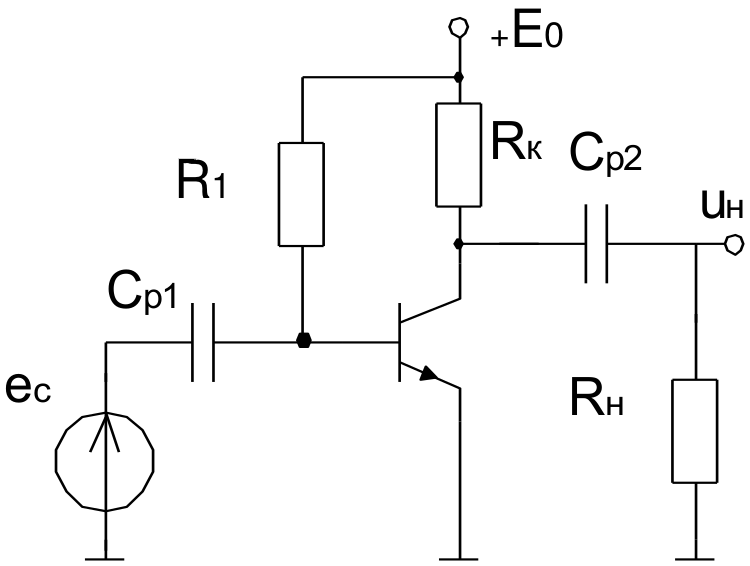
\includegraphics[width=7cm]{img/scheme}
		\caption{Схема однокаскадного усилителя}
		\label{figure:1}
	\vspace{-0.5cm}
	\end{center}
\end{figure}

\section{Исходные данные}

Транзистор МП39. Кремниевый транзистор с $p-n-p$ переходом.

\begin{table}[H]
	\begin{center}
	\caption{Исходные данные}
	\def\arraystretch{1.4}
		\begin{tabularx}{\textwidth}{|X|X|X|X|X|X|X|X|X|X|}
			\hline
			$E_0$ &
			$U_\text{кэА}$ &
			$U_\text{бэ}$ &
			$R_\text{к}$ &
			$R_\text{н}$ &
			$C_{p1}$ &
			$C_{p2}$ &
			$f_{h21}$ &
			$C_\text{к}$ &
			$h_{21}$ \\
			\hline
			В &
			В &
			В &
			кОм &
			кОм &
			мкФ &
			мкФ &
			МГц &
			пФ &
			\\
			\hline
			8 &
			4 &
			0.2 &
			3.9 &
			2 &
			0.22 &
			0.47 &
			0.5 &
			60 &
			12 \\
		    \hline	
		\end{tabularx}
		\label{tabular:1}
	\end{center}
\end{table}

\section{Теоретические расчёты}

\section{Экспериментально снятые зависимости}

\subsection{Амплитудная характеристика усилителя}

В таблице \ref{tabular:2} приведена амплитудная характеристика усилителя\\ $U_\text{вых} = f(e_c)$. При значениях $e_c > e_{max} = 30.1$ можно заметить искажение входного сигнала. По полученным значениям было вычислено значение коэффициента усиления $K = 55.94$.

\begin{table}[H]
	\begin{center}
	\caption{Зависимость напряжения $U_\text{вых}$ от $e_c$}
	\def\arraystretch{1.2}
		\begin{tabularx}{\textwidth}{|X|X|X|}
			\hline
			$e_c$, мВ & $U_\text{вых}$, мВ & $K$ \\\hline			
			1.43 & 90.1 & 63.01\\\hline	
			3.09 & 200 & 64.72\\\hline	
			5.07 & 324 & 63.91\\\hline	
			7.54 & 476 & 63.13\\\hline	
			10.7 & 675 & 63.08\\\hline	
			13.1 & 799 & 60.99\\\hline	
			15.2 & 913 & 60.07\\\hline	
			17.7 & 1053 & 59.49\\\hline	
			20.7 & 1190 & 57.49\\\hline	
			23.1 & 1310 & 56.71\\\hline	
			25.3 & 1390 & 54.94\\\hline	
			27.9 & 1490 & 53.41\\\hline	
			30.1 & 1580 & 52.49\\\hline\hline	
			33.1 & 1690 & 51.06\\\hline	
			35.9 & 1750 & 48.75\\\hline	
			39.6 & 1830 & 46.21\\\hline	
			43.1 & 1910 & 44.32\\\hline	
			45.9 & 1980 & 43.14\\\hline
		\end{tabularx}
		\label{tabular:2}
	\end{center}
\end{table}

\begin{figure}[H]
	\begin{center}
		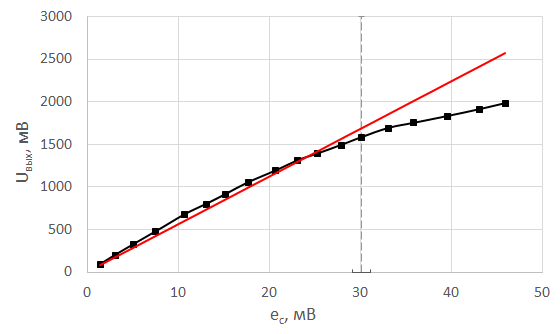
\includegraphics[height=9cm]{img/1}
		\caption{Зависимость напряжения $U_\text{вых}$ от $e_c$}
		\label{figure:2}
	\end{center}
\end{figure}

\subsection{Логарифмическая амплитудно-частотная характеристика усилителя}

В таблице \ref{tabular:3} приведена амплитудно-частотная характеристика усилителя при $e_c = \frac{e_{max}}{2} \approx 20$ мВ.

\begin{table}[H]
	\begin{center}
	\caption{ЛАЧХ усилителя}
	\def\arraystretch{1.2}
		\begin{tabularx}{\textwidth}{|X|X|X|X|}
			\hline
			$f$, Гц & $U_\text{вых}$, В & $K$ & $20 \cdot lg(K)$, дБ\\\hline
			16 & 5.07 & 0.2535 & -11.9204\\\hline	
			32 & 17.2 & 0.86 & -1.3100\\\hline	
			64 & 49.7 & 2.485 & 7.9065\\\hline	
			128 & 119 & 5.95 & 15.4903\\\hline	
			256 & 238 & 11.9 & 21.5109\\\hline	
			512 & 415 & 20.75 & 26.3404\\\hline	
			1024 & 558 & 27.9 & 28.9121\\\hline	
			2048 & 623 & 31.15 & 29.8692\\\hline	
			4096 & 639 & 31.95 & 30.0894\\\hline	
			8192 & 641 & 32.05 & 30.1166\\\hline	
			16384 & 638 & 31.9 & 30.0758\\\hline	
			32768 & 625 & 31.25 & 29.8970\\\hline	
			65536 & 612 & 30.6 & 29.7144\\\hline	
			131072 & 587 & 29.35 & 29.3522\\\hline	
			200000 & 557 & 27.85 & 28.8965\\\hline	
		\end{tabularx}
		\label{tabular:3}
	\end{center}
\end{table}

\begin{figure}[H]
	\begin{center}
		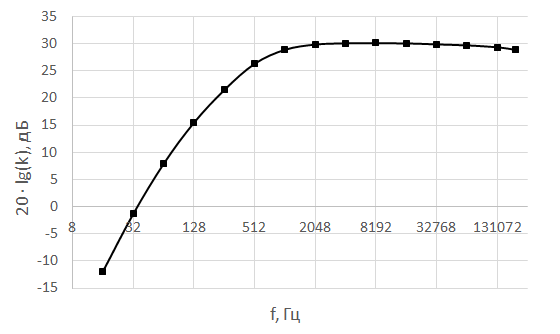
\includegraphics[height=9cm]{img/2}
		\caption{\textbf{Добавить теорию} ЛАЧХ усилителя}
		\label{figure:2}
	\end{center}
\end{figure}

\section{Уточнение теоретических величин}

\section{Выводы}

\end{document}
